\chapter[Questionários]{Questionários}
\label{chap:questionarios}
	
	Os questinários guiam a avaliação de protótipos com os usuários tratando-se de um objeto muito importante durante a fase de teste para a aplicação. Para o projeto, foram avaliação 3 grupos de questinários conhecidos. São eles:

	\begin{itemize}
			\item{QUIS;}
			\item{SUMI;}
			\item{ErgoList.}
		\end{itemize}

	\begin{flushleft}
		Nas seções a seguir serão apresentadas os estudos avaliativos dessas ferramentas.
	\end{flushleft}

	\section[QUIS]{QUIS - \emph{Questionnaire for User Interaction Satisfaction}}
	\label{sec:questionarios_QUIS}

		\begin{figure}[h]
			\centering
			
\includegraphics[scale=0.5]{logo1}
			\caption[Logo QUIS]{Logo QUIS. \cite{quis}}
			\label{fig:logo1}
		\end{figure}

		Mede a satisfação do usuário quanto à usabilidade do produto, de maneira padronizada, segura e válida. Obtém informações precisas em relação à reação dos usuários a novos produtos. 

		\textbf{Histórico}

		\begin{itemize}
			\item{Desenvolvido por um grupo de pesquisadores da Human/Computer Interaction Laboratory at the University of Maryland;}
			\item{O questionário original (MEDEIROS, 1999) consistia de noventa perguntas;}
			\item{Na 2ª versão foram inseridas mais treze perguntas e foi modificada a escala de 1 a 10 para 1 a 9, pois neste caso pode-se incluir o 0 como não aplicável;}
			\item{O QUIS é continuamente atualizado e refinado para vários ambientes acadêmicos e industriais. Atualmente está na versão 7.0.}
		\end{itemize}

		\textbf{Estrutura}

		Hierarquicamente organizado em sete fatores referentes à interface: 

		\begin{itemize}
			\item{Fatores relacionados às telas;}
			\item{Terminologia e retorno do sistema;}
			\item{Fatores relacionados ao aprendizado;}
			\item{Capacidade do sistema;}
			\item{Manuais técnicos;}
			\item{Tutoriais on-line;}
			\item{Multimídia;}
			\item{Reconhecimento de voz;}
			\item{Ambientes virtuais;}
			\item{Acesso à Internet;}
			\item{Instalação do software.}
		\end{itemize}

		\textbf{Finalidade do questionário}

		Guiar no projeto ou no redesign dos sistemas. 
		Dar a gerentes uma ferramenta para que possam avaliar áreas potenciais de melhoria do sistema. 
		Fornecer investigadores de um instrumento validado que conduz a avaliações comparativas e serve como uma ferramenta de teste em laboratórios .

		Além do mais, possui as vantagens de alta confiabilidade, baixa variabilidade e informações para projetistas. 

	\section[SUMI]{SUMI - \emph{Software Usability Measurement Inventory}}
	\label{sec:questionarios_SUMI}

		\begin{figure}[h]
			\centering
			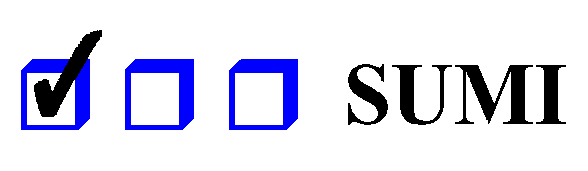
\includegraphics[scale=0.4]{logo2}
			\caption[Logo SUMI]{Logo SUMI. \cite{sumi}}
			\label{fig:logo2}
		\end{figure}

		É recomendado a qualquer organização ou consumidor que deseja medir a qualidade de uso de softwares. Os usuários usam-no efetivamente para: 

		\begin{itemize}
			\item{Calcular o valor de produtos novos durante avaliação desse produto;}
			\item{Fazer comparações entre produtos ou versões de produtos;}
			\item{Fixar objetivos para desenvolvimento de aplicações futuras;}
			\item{Identificar o software mais apropriado para sua organização.}
		\end{itemize}

		Usa-se SUMI especificamente dentro de ambientes de desenvolvimento para:

		\begin{itemize}
			\item{Estabelecer metas verificáveis para qualidade de consentimento de uso;}
			\item{Localizar realização de objetivos durante o desenvolvimento de produto;}
			\item{Realçar aspectos bons e ruins de uma interface.}
		\end{itemize}

		\textbf{Vantagens}

		SUMI é o único questionário comercialmente disponível para a avaliação da usabilidade de software desenvolvido, validado e unificado em uma base internacional. 

		Está disponível em grande número de idiomas cujas versões são traduzidas e validadas. A \textbf{ISO 9241} menciona que o SUMI é um reconhecido método para testar a satisfação do usuário que consiste em cinquenta declarações nas quais o usuário escolhe entre as alternativas Concordam, Não sabem ou Discordam. \cite{iso}

	\section[ErgoList]{ErgoList}
	\label{sec:questionarios_ErgoList}

		\begin{figure}[h]
			\centering
			
\includegraphics[scale=0.6]{logo3}
			\caption[Logo ErgoList]{Logo ErgoList.\cite{ergoList}}
			\label{fig:logo2}
		\end{figure}

		O ErgoList é destinado às pessoas que possuem interesse em melhorias na intuitividade, na facilidade de uso e na utilidade dos programas de software interativos. Assim sendo, o ErgoList pode iniciar o conhecimento na técnica de inspeção da ergonomia de interfaces homem-máquina.
		
		O maior objetivo do ErgoList, segundo pesquisadores da Universidade Federal de Santa Catarina, é levar o estudante a descobrir as falhas ergonômicas mais flagrantes em uma interface com o usuário, conferindo ao ErgoList uma caracterização didática.
		
		Para aprofundamento de avaliações de ergonomia e interface, a \textbf{ISO 9241} confere uma série de diretrizes. \cite{iso}

		O ErgoList apresenta os seguintes módulos: 

		\begin{itemize}
			\item{\textbf{Checklist} – esse módulo irá auxiliá-lo a realizar uma inspeção da qualidade ergonômica da interface com o usuário de seu sistema;}
			\item{\textbf{Questões} – esse módulo fornece a possibilidade de conhecer, de maneira informal, as questões que compõem o módulo Checklist;}
			\item{\textbf{Recomendações} – esse módulo apresenta recomendações ergonômicas que podem auxiliá-lo nas decisões de projeto de interfaces com o usuário.}
		\end{itemize}

		É importante ressaltar que o LabIUtil, idealizador do ErgoList, tomou iniciativas importantes a favor da usabilidade de interfaces humano-computador. Esteve envolvido com a montagem da comissão de estudos da ABNT para elaboração da norma brasileira sobre ergonomia do trabalho de escritório com computadores (\textbf{NBR 9241}).

		\label{subsubsec:questionarios_tables}
		\begin{table}[h]
			\centering 
			\begin{tabular}{|c|c|c|c|}

				\hline

				Tipo & Preço & Estudante\footnotemark[1] & Free \\
				
				\hline
				
				QUIS & \$750 & \$50 & Não \\
				
				SUMI & \$1600 - \$3200 & Sim & Não \\
				
				ErgoList & Free & --- & Sim  \\

				\hline

			\end{tabular}
			\caption[Tabela comparativa de Preços - Questionários de Avaliação]{Tabela comparativa de Preços - Questionários de Avaliação.}
			\label{tab:questionarios._tabl}
		\end{table}

		\footnotetext[1]{Para obter versão estudante das ferramentas é necessário contato com a empresa fornecedora do serviço. Cada uma possui um procedimento específico de contato.}



		

		

